\documentclass[10pt, a4paper]{article}
\usepackage[utf8]{inputenc}
 
\usepackage[danish]{babel}
\usepackage{blindtext}
\usepackage[hidelinks]{hyperref}
\usepackage{graphicx}
\usepackage{caption}
\usepackage{subcaption}
\usepackage{xcolor}
\usepackage{url}
\usepackage[margin=1in]{geometry}
\usepackage[square,comma,numbers]{natbib}
\usepackage{float}

\begin{document}

\section{Exo-Aider armband update}

This document will give an update on the progress of the data-collection armband in the Exo-Aider project. The development of the armband is currently stalled because of the current COVID-19 situation. 



\subsection{Hardware}
The first revision of the hardware (filters, SPI connections and DAC/ADC) have been debugged and tested through with good results and some changes to the hardware. The next revision of the hardware is already designed and the pin-out of the PCB is in progress. Hopefully the next revision of the hardware will be ready to test when the we get back at the university.  


\subsection{Armband}
To make the armband easy to attach it is being build around a blood pressure armband as shown in \autoref{fig:armband}. This also makes it easier to attach yourself and by that also makes it easier to test by yourself. 

\begin{figure}[htbp]
    \centering
    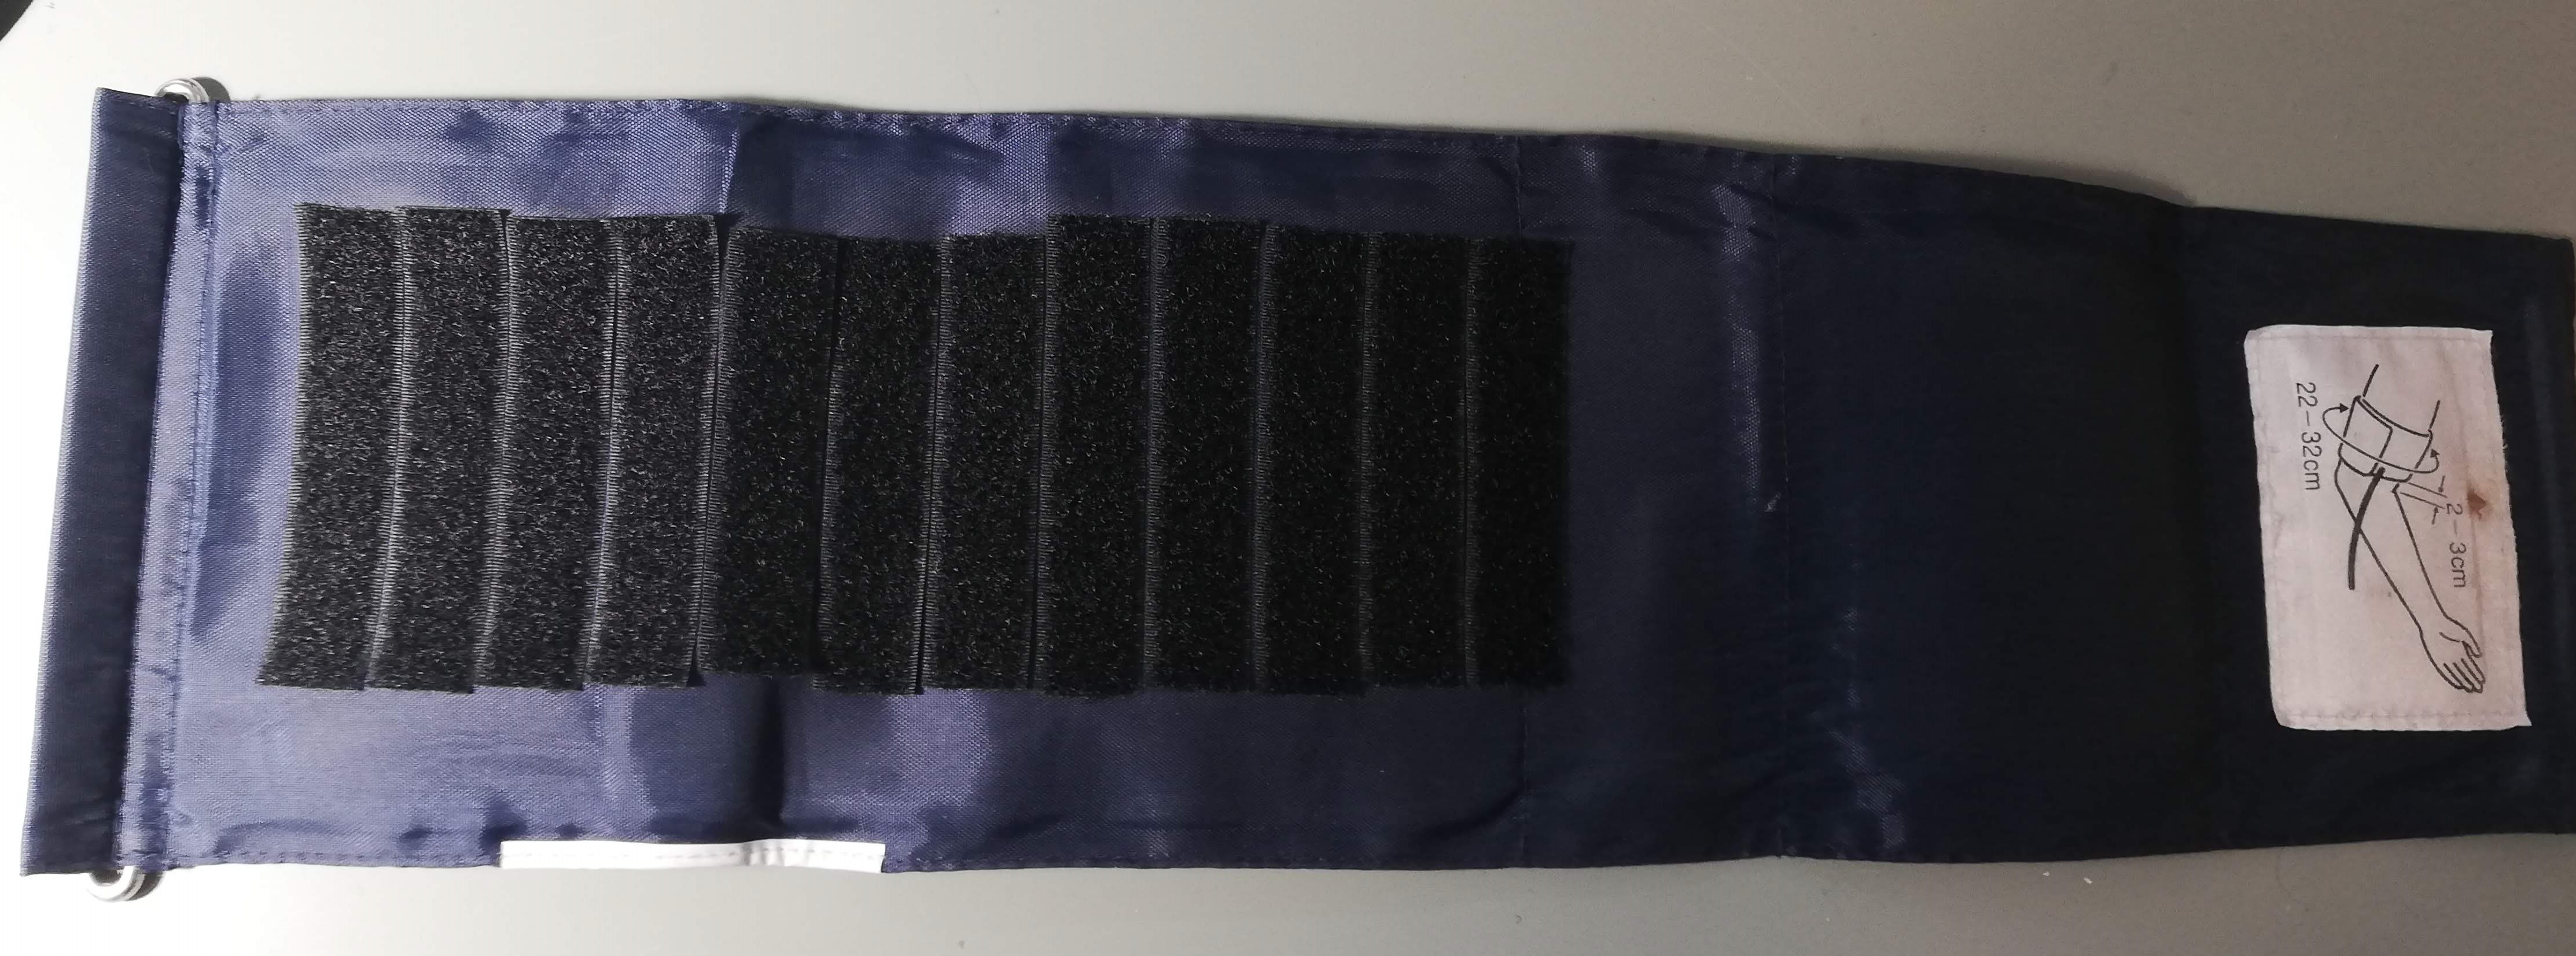
\includegraphics[width=0.8\textwidth]{figures/armband.jpg}
    \caption{Blood pressure armband with Velcro}
    \label{fig:armband}
\end{figure}

The sensors will be build into two modules consisting of four FSR sensors and two sEMG sensors for each module as shown on \autoref{fig:onmodule} which show the concept of the module since the materials for finishing the modules are not available at the moment. 

\begin{figure}[htbp]
    \centering
    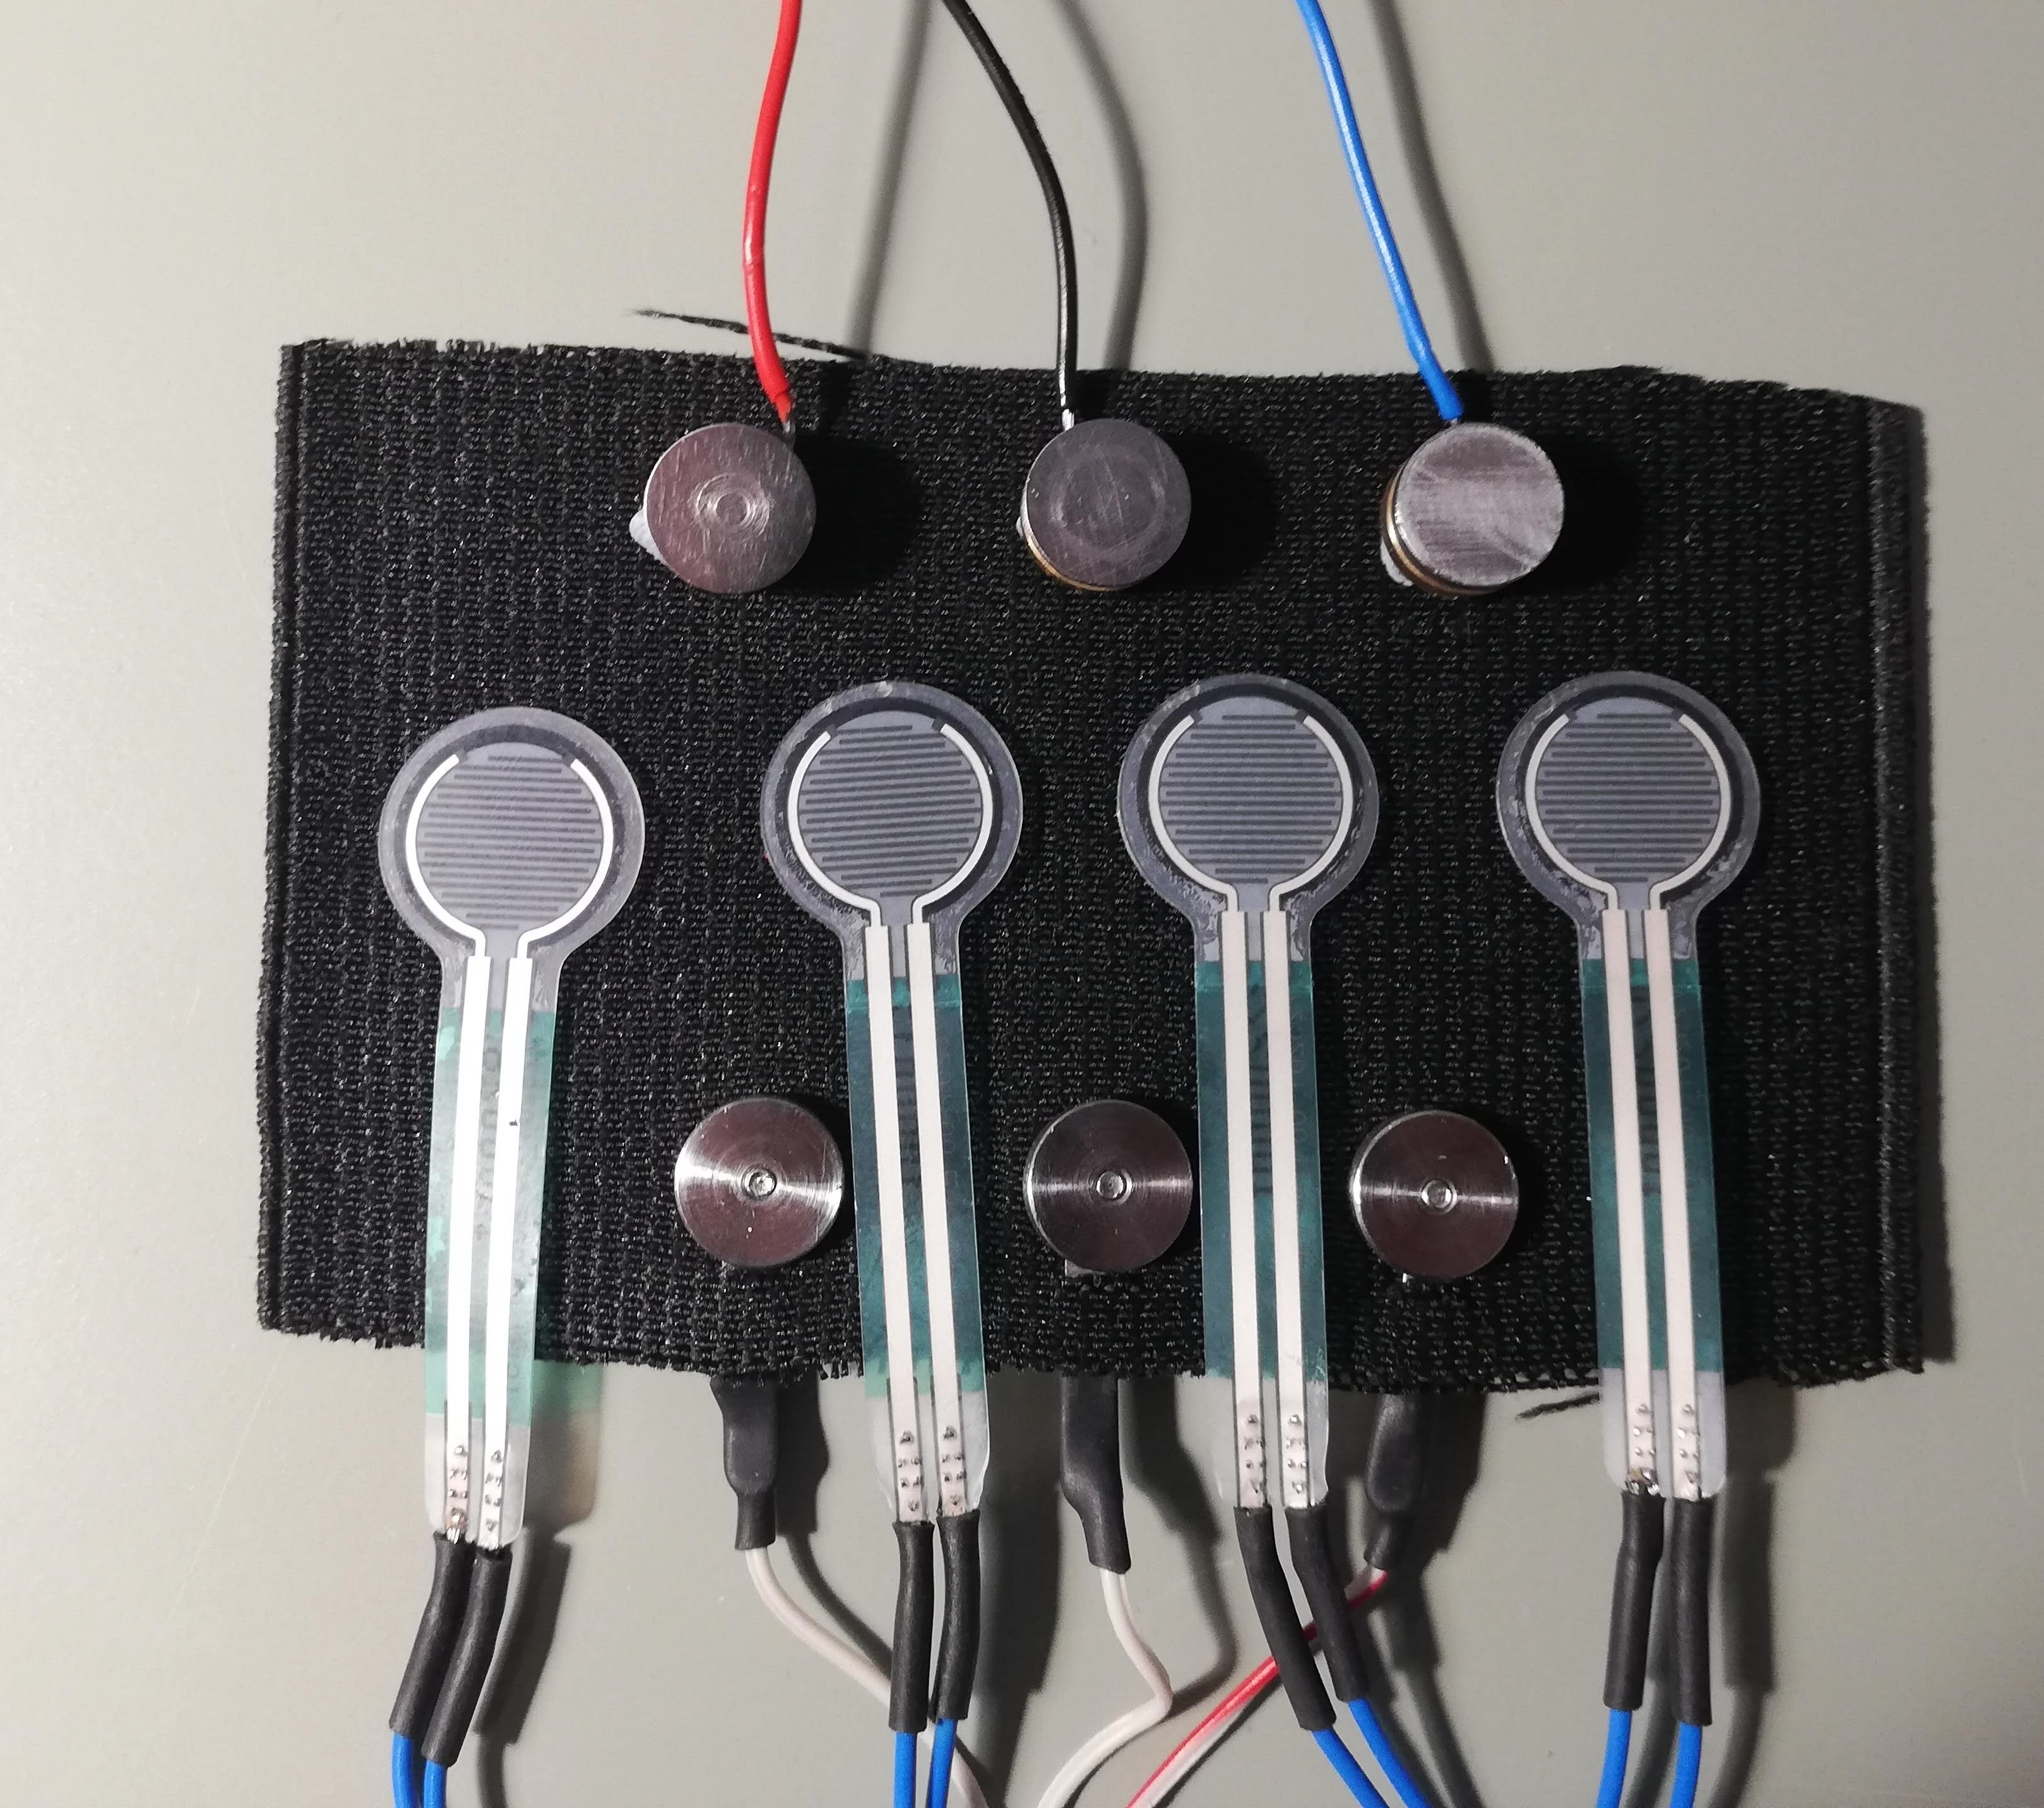
\includegraphics[width=0.4\textwidth]{figures/one_module.jpg}
    \caption{One module consisting of four FSR sensors and two sEMG sensors}
    \label{fig:onmodule}
\end{figure}

By making the armband modular it is possible to move each module around to target the biceps and the triceps of each individual but still keep the same orientation between the sensors in the module. The idea of this is to keep everything as consistent as possible between different people. 


Finally, the armband is almost ready to be combined with the rest of the exoskeleton as soon as the new hardware has been manufactured and tested and the sensors are mounted on the modules.

\subsection{Software}
To ensure a stable transmission of data from the armband to Matlab, new code for the Bluetooth connection was created. It is intended to sample with at least 1 kHz from the sensors on the armband to be able to sample frequencies up to 500 Hz, and since Bluetooth has a polling rate up to 125 Hz, a configuration to ensure that all the data is transmitted had to be made. The previously used code sent the data as fast as possible to Matlab, but it was not possible to monitor this rate. The code could be used to test and verify sensor data, but for further work where stability and the timestamp of the measurement has to be know, the code was not useable.

The new solution is made with the possibility to choose a high or a low sampling rate, which can be set from Matlab, to reduce the bandwidth required. This makes it possible to sample sensors that need higher sample rates with one rate (e.g. sEMG) and ones that does not need as high sample rate with another (e.g. FSR).

The way this is implemented is to batch the data and sending it via Bluetooth at a rate lower than 125 Hz. The high frequency batches include all the data sampled at a rate equal or higher than 1 kHz and the low frequency batch contains data sampled at a lower rate. The principle is shown in \autoref{tab:sampling_principle}.

\begin{table}[htbp]
\centering
\caption{High and low frequency sampling principle}
\label{tab:sampling_principle}
\begin{tabular}{|l|lll|lll|lll|lll|}
\hline
\textbf{Transmission number} &
  \multicolumn{3}{c|}{\textbf{1}} &
  \multicolumn{3}{c|}{\textbf{2}} &
  \multicolumn{3}{c|}{\textbf{3}} &
  \multicolumn{3}{c|}{\textbf{4}} \\ \hline
\textbf{High frequency sampling} &
  \cellcolor[HTML]{9B9B9B}1 &
  \cellcolor[HTML]{9B9B9B}2 &
  \cellcolor[HTML]{9B9B9B}3 &
  \cellcolor[HTML]{9B9B9B}4 &
  \cellcolor[HTML]{9B9B9B}5 &
  \cellcolor[HTML]{9B9B9B}6 &
  \cellcolor[HTML]{9B9B9B}7 &
  \cellcolor[HTML]{9B9B9B}8 &
  \cellcolor[HTML]{9B9B9B}9 &
  \cellcolor[HTML]{9B9B9B}10 &
  \cellcolor[HTML]{9B9B9B}11 &
  \cellcolor[HTML]{9B9B9B}12 \\
\textbf{Low frequency sampling} &
  \cellcolor[HTML]{9B9B9B}1 &
  1 &
  1 &
  \cellcolor[HTML]{9B9B9B}4 &
  4 &
  4 &
  \cellcolor[HTML]{9B9B9B}7 &
  7 &
  7 &
  \cellcolor[HTML]{9B9B9B}10 &
  10 &
  10 \\ \hline
\end{tabular}
\end{table}

The new software has been tested with a sine signal which shows that the program does as intended, but it has not been tested with the sensors and hardware since it is locked in at the University due to the COVID-19 lockdown. The sensor reading and processing is implemented from the existing solution, and it should be possible to test as soon as the hardware is available again.


\end{document}